% Options for packages loaded elsewhere
\PassOptionsToPackage{unicode}{hyperref}
\PassOptionsToPackage{hyphens}{url}
\documentclass[
  11pt,
]{article}
\usepackage{xcolor}
\usepackage[margin=1in]{geometry}
\usepackage{amsmath,amssymb}
\setcounter{secnumdepth}{5}
\usepackage{iftex}
\ifPDFTeX
  \usepackage[T1]{fontenc}
  \usepackage[utf8]{inputenc}
  \usepackage{textcomp} % provide euro and other symbols
\else % if luatex or xetex
  \usepackage{unicode-math} % this also loads fontspec
  \defaultfontfeatures{Scale=MatchLowercase}
  \defaultfontfeatures[\rmfamily]{Ligatures=TeX,Scale=1}
\fi
\usepackage{lmodern}
\ifPDFTeX\else
  % xetex/luatex font selection
\fi
% Use upquote if available, for straight quotes in verbatim environments
\IfFileExists{upquote.sty}{\usepackage{upquote}}{}
\IfFileExists{microtype.sty}{% use microtype if available
  \usepackage[]{microtype}
  \UseMicrotypeSet[protrusion]{basicmath} % disable protrusion for tt fonts
}{}
\makeatletter
\@ifundefined{KOMAClassName}{% if non-KOMA class
  \IfFileExists{parskip.sty}{%
    \usepackage{parskip}
  }{% else
    \setlength{\parindent}{0pt}
    \setlength{\parskip}{6pt plus 2pt minus 1pt}}
}{% if KOMA class
  \KOMAoptions{parskip=half}}
\makeatother
\usepackage{color}
\usepackage{fancyvrb}
\newcommand{\VerbBar}{|}
\newcommand{\VERB}{\Verb[commandchars=\\\{\}]}
\DefineVerbatimEnvironment{Highlighting}{Verbatim}{commandchars=\\\{\}}
% Add ',fontsize=\small' for more characters per line
\usepackage{framed}
\definecolor{shadecolor}{RGB}{248,248,248}
\newenvironment{Shaded}{\begin{snugshade}}{\end{snugshade}}
\newcommand{\AlertTok}[1]{\textcolor[rgb]{0.94,0.16,0.16}{#1}}
\newcommand{\AnnotationTok}[1]{\textcolor[rgb]{0.56,0.35,0.01}{\textbf{\textit{#1}}}}
\newcommand{\AttributeTok}[1]{\textcolor[rgb]{0.13,0.29,0.53}{#1}}
\newcommand{\BaseNTok}[1]{\textcolor[rgb]{0.00,0.00,0.81}{#1}}
\newcommand{\BuiltInTok}[1]{#1}
\newcommand{\CharTok}[1]{\textcolor[rgb]{0.31,0.60,0.02}{#1}}
\newcommand{\CommentTok}[1]{\textcolor[rgb]{0.56,0.35,0.01}{\textit{#1}}}
\newcommand{\CommentVarTok}[1]{\textcolor[rgb]{0.56,0.35,0.01}{\textbf{\textit{#1}}}}
\newcommand{\ConstantTok}[1]{\textcolor[rgb]{0.56,0.35,0.01}{#1}}
\newcommand{\ControlFlowTok}[1]{\textcolor[rgb]{0.13,0.29,0.53}{\textbf{#1}}}
\newcommand{\DataTypeTok}[1]{\textcolor[rgb]{0.13,0.29,0.53}{#1}}
\newcommand{\DecValTok}[1]{\textcolor[rgb]{0.00,0.00,0.81}{#1}}
\newcommand{\DocumentationTok}[1]{\textcolor[rgb]{0.56,0.35,0.01}{\textbf{\textit{#1}}}}
\newcommand{\ErrorTok}[1]{\textcolor[rgb]{0.64,0.00,0.00}{\textbf{#1}}}
\newcommand{\ExtensionTok}[1]{#1}
\newcommand{\FloatTok}[1]{\textcolor[rgb]{0.00,0.00,0.81}{#1}}
\newcommand{\FunctionTok}[1]{\textcolor[rgb]{0.13,0.29,0.53}{\textbf{#1}}}
\newcommand{\ImportTok}[1]{#1}
\newcommand{\InformationTok}[1]{\textcolor[rgb]{0.56,0.35,0.01}{\textbf{\textit{#1}}}}
\newcommand{\KeywordTok}[1]{\textcolor[rgb]{0.13,0.29,0.53}{\textbf{#1}}}
\newcommand{\NormalTok}[1]{#1}
\newcommand{\OperatorTok}[1]{\textcolor[rgb]{0.81,0.36,0.00}{\textbf{#1}}}
\newcommand{\OtherTok}[1]{\textcolor[rgb]{0.56,0.35,0.01}{#1}}
\newcommand{\PreprocessorTok}[1]{\textcolor[rgb]{0.56,0.35,0.01}{\textit{#1}}}
\newcommand{\RegionMarkerTok}[1]{#1}
\newcommand{\SpecialCharTok}[1]{\textcolor[rgb]{0.81,0.36,0.00}{\textbf{#1}}}
\newcommand{\SpecialStringTok}[1]{\textcolor[rgb]{0.31,0.60,0.02}{#1}}
\newcommand{\StringTok}[1]{\textcolor[rgb]{0.31,0.60,0.02}{#1}}
\newcommand{\VariableTok}[1]{\textcolor[rgb]{0.00,0.00,0.00}{#1}}
\newcommand{\VerbatimStringTok}[1]{\textcolor[rgb]{0.31,0.60,0.02}{#1}}
\newcommand{\WarningTok}[1]{\textcolor[rgb]{0.56,0.35,0.01}{\textbf{\textit{#1}}}}
\usepackage{graphicx}
\makeatletter
\newsavebox\pandoc@box
\newcommand*\pandocbounded[1]{% scales image to fit in text height/width
  \sbox\pandoc@box{#1}%
  \Gscale@div\@tempa{\textheight}{\dimexpr\ht\pandoc@box+\dp\pandoc@box\relax}%
  \Gscale@div\@tempb{\linewidth}{\wd\pandoc@box}%
  \ifdim\@tempb\p@<\@tempa\p@\let\@tempa\@tempb\fi% select the smaller of both
  \ifdim\@tempa\p@<\p@\scalebox{\@tempa}{\usebox\pandoc@box}%
  \else\usebox{\pandoc@box}%
  \fi%
}
% Set default figure placement to htbp
\def\fps@figure{htbp}
\makeatother
\setlength{\emergencystretch}{3em} % prevent overfull lines
\providecommand{\tightlist}{%
  \setlength{\itemsep}{0pt}\setlength{\parskip}{0pt}}
\usepackage{amsmath}
% Shared LaTeX preamble for all Data Mining / ISLR chapter documents.
% Provides \makecoverpage{<assignment title>} — a standalone title page
% with fixed student identity, so every chapter/lab looks uniform.

\usepackage{graphicx}

\newcommand{\makecoverpage}[1]{%
\begin{titlepage}
\centering
\vspace*{2cm}

{\Large \textbf{Adventist University of Central Africa}}\\[0.4cm]
{\large Master's in Big Data Analytics}\\[2cm]

{\Huge \textbf{#1}}\\[0.5cm]
{\large \textit{Introduction to Statistical Learning with Applications in R}}\\[3cm]

\begin{tabular}{rl}
\textbf{Programme:} & MSc Big Data Analytics \\
\textbf{Course Title:} & Data Mining \\
\textbf{Course Code:} & MSDA 9124 \\
\textbf{Lecturer:} & Dr. Pacifique Nizeyimana \\
\textbf{Student Name:} & Wayne Rubangisa \\
\textbf{Student ID:} & 101220 \\
\end{tabular}

\vfill

{\large September 2026}

\end{titlepage}
}

\usepackage{bookmark}
\IfFileExists{xurl.sty}{\usepackage{xurl}}{} % add URL line breaks if available
\urlstyle{same}
\hypersetup{
  hidelinks,
  pdfcreator={LaTeX via pandoc}}

\author{}
\date{\vspace{-2.5em}}

\begin{document}

\makecoverpage{Chapter 8 --- Tree-Based Methods \\ Lab}

\section{Introduction}\label{introduction}

A decision tree predicts an outcome by repeatedly splitting the
predictor space into simpler regions. The result is easy to explain:
observations that follow the same sequence of splits receive the same
prediction. Trees are therefore attractive when interpretability,
nonlinear relationships, and interactions matter.

Their main weakness is instability. A small change in the training data
can change an early split, which can change the entire tree below it.
This lab starts with individual classification and regression trees,
then introduces three ensemble approaches that address this instability
in different ways:

\begin{enumerate}
\def\labelenumi{\arabic{enumi}.}
\tightlist
\item
  pruning controls the complexity of one tree;
\item
  Bagging averages many trees trained on bootstrap samples;
\item
  Random Forests add random feature selection to reduce correlation
  between the trees; and
\item
  Boosting builds trees sequentially to correct the current model's
  errors.
\end{enumerate}

The lab follows the Chapter 8.3 workflow from \emph{An Introduction to
Statistical Learning}. The explanations state the practical idea first
and then connect it to the relevant statistical objective.

\begin{Shaded}
\begin{Highlighting}[]
\CommentTok{\# Install these once if necessary:}
\CommentTok{\# install.packages(c("ISLR2", "tree", "randomForest", "gbm", "BART"))}

\FunctionTok{library}\NormalTok{(ISLR2)}
\FunctionTok{library}\NormalTok{(tree)}
\FunctionTok{library}\NormalTok{(randomForest)}
\FunctionTok{library}\NormalTok{(gbm)}
\FunctionTok{library}\NormalTok{(BART)}
\end{Highlighting}
\end{Shaded}

\section{Classification Trees}\label{classification-trees}

\subsection{\texorpdfstring{The \texttt{Carseats}
data}{The Carseats data}}\label{the-carseats-data}

The \texttt{Carseats} data describe the sales of child car seats at 400
stores. Our first task is classification: we create a binary response
indicating whether sales are high or low.

A store is labelled \texttt{Yes} when \texttt{Sales} exceeds 8 thousand
units and \texttt{No} otherwise. This threshold is a modelling choice:
it changes a continuous business outcome into a decision problem that
could support an action such as identifying stores for extra promotion.

\begin{Shaded}
\begin{Highlighting}[]
\FunctionTok{data}\NormalTok{(Carseats)}
\NormalTok{High }\OtherTok{\textless{}{-}} \FunctionTok{factor}\NormalTok{(}\FunctionTok{ifelse}\NormalTok{(Carseats}\SpecialCharTok{$}\NormalTok{Sales }\SpecialCharTok{\textless{}=} \DecValTok{8}\NormalTok{, }\StringTok{"No"}\NormalTok{, }\StringTok{"Yes"}\NormalTok{))}
\NormalTok{Carseats }\OtherTok{\textless{}{-}} \FunctionTok{data.frame}\NormalTok{(Carseats, High)}

\FunctionTok{str}\NormalTok{(Carseats)}
\end{Highlighting}
\end{Shaded}

\begin{verbatim}
## 'data.frame':    400 obs. of  12 variables:
##  $ Sales      : num  9.5 11.22 10.06 7.4 4.15 ...
##  $ CompPrice  : num  138 111 113 117 141 124 115 136 132 132 ...
##  $ Income     : num  73 48 35 100 64 113 105 81 110 113 ...
##  $ Advertising: num  11 16 10 4 3 13 0 15 0 0 ...
##  $ Population : num  276 260 269 466 340 501 45 425 108 131 ...
##  $ Price      : num  120 83 80 97 128 72 108 120 124 124 ...
##  $ ShelveLoc  : Factor w/ 3 levels "Bad","Good","Medium": 1 2 3 3 1 1 3 2 3 3 ...
##  $ Age        : num  42 65 59 55 38 78 71 67 76 76 ...
##  $ Education  : num  17 10 12 14 13 16 15 10 10 17 ...
##  $ Urban      : Factor w/ 2 levels "No","Yes": 2 2 2 2 2 1 2 2 1 1 ...
##  $ US         : Factor w/ 2 levels "No","Yes": 2 2 2 2 1 2 1 2 1 2 ...
##  $ High       : Factor w/ 2 levels "No","Yes": 2 2 2 1 1 2 1 2 1 1 ...
\end{verbatim}

\begin{Shaded}
\begin{Highlighting}[]
\FunctionTok{table}\NormalTok{(Carseats}\SpecialCharTok{$}\NormalTok{High)}
\end{Highlighting}
\end{Shaded}

\begin{verbatim}
## 
##  No Yes 
## 236 164
\end{verbatim}

\subsection{Growing a classification
tree}\label{growing-a-classification-tree}

A classification tree partitions the predictor space into regions and
assigns one class to each terminal region. At a candidate split, the
algorithm looks for a partition that makes the resulting child nodes
purer. One common purity measure is the Gini index:

\[
G = \sum_{k=1}^{K} \hat p_k(1-\hat p_k),
\]

where \(\hat p_k\) is the proportion of observations in the node
belonging to class \(k\). A node containing only one class has Gini
index zero; a mixed node has a larger value.

The \texttt{tree()} function grows a large tree first. This is useful
because the subsequent pruning step can compare smaller subtrees
obtained from the large candidate tree.

\begin{Shaded}
\begin{Highlighting}[]
\NormalTok{tree.carseats }\OtherTok{\textless{}{-}} \FunctionTok{tree}\NormalTok{(High }\SpecialCharTok{\textasciitilde{}}\NormalTok{ . }\SpecialCharTok{{-}}\NormalTok{ Sales, }\AttributeTok{data =}\NormalTok{ Carseats)}
\NormalTok{tree.carseats}
\end{Highlighting}
\end{Shaded}

\begin{verbatim}
## node), split, n, deviance, yval, (yprob)
##       * denotes terminal node
## 
##   1) root 400 541.500 No ( 0.59000 0.41000 )  
##     2) ShelveLoc: Bad,Medium 315 390.600 No ( 0.68889 0.31111 )  
##       4) Price < 92.5 46  56.530 Yes ( 0.30435 0.69565 )  
##         8) Income < 57 10  12.220 No ( 0.70000 0.30000 )  
##          16) CompPrice < 110.5 5   0.000 No ( 1.00000 0.00000 ) *
##          17) CompPrice > 110.5 5   6.730 Yes ( 0.40000 0.60000 ) *
##         9) Income > 57 36  35.470 Yes ( 0.19444 0.80556 )  
##          18) Population < 207.5 16  21.170 Yes ( 0.37500 0.62500 ) *
##          19) Population > 207.5 20   7.941 Yes ( 0.05000 0.95000 ) *
##       5) Price > 92.5 269 299.800 No ( 0.75465 0.24535 )  
##        10) Advertising < 13.5 224 213.200 No ( 0.81696 0.18304 )  
##          20) CompPrice < 124.5 96  44.890 No ( 0.93750 0.06250 )  
##            40) Price < 106.5 38  33.150 No ( 0.84211 0.15789 )  
##              80) Population < 177 12  16.300 No ( 0.58333 0.41667 )  
##               160) Income < 60.5 6   0.000 No ( 1.00000 0.00000 ) *
##               161) Income > 60.5 6   5.407 Yes ( 0.16667 0.83333 ) *
##              81) Population > 177 26   8.477 No ( 0.96154 0.03846 ) *
##            41) Price > 106.5 58   0.000 No ( 1.00000 0.00000 ) *
##          21) CompPrice > 124.5 128 150.200 No ( 0.72656 0.27344 )  
##            42) Price < 122.5 51  70.680 Yes ( 0.49020 0.50980 )  
##              84) ShelveLoc: Bad 11   6.702 No ( 0.90909 0.09091 ) *
##              85) ShelveLoc: Medium 40  52.930 Yes ( 0.37500 0.62500 )  
##               170) Price < 109.5 16   7.481 Yes ( 0.06250 0.93750 ) *
##               171) Price > 109.5 24  32.600 No ( 0.58333 0.41667 )  
##                 342) Age < 49.5 13  16.050 Yes ( 0.30769 0.69231 ) *
##                 343) Age > 49.5 11   6.702 No ( 0.90909 0.09091 ) *
##            43) Price > 122.5 77  55.540 No ( 0.88312 0.11688 )  
##              86) CompPrice < 147.5 58  17.400 No ( 0.96552 0.03448 ) *
##              87) CompPrice > 147.5 19  25.010 No ( 0.63158 0.36842 )  
##               174) Price < 147 12  16.300 Yes ( 0.41667 0.58333 )  
##                 348) CompPrice < 152.5 7   5.742 Yes ( 0.14286 0.85714 ) *
##                 349) CompPrice > 152.5 5   5.004 No ( 0.80000 0.20000 ) *
##               175) Price > 147 7   0.000 No ( 1.00000 0.00000 ) *
##        11) Advertising > 13.5 45  61.830 Yes ( 0.44444 0.55556 )  
##          22) Age < 54.5 25  25.020 Yes ( 0.20000 0.80000 )  
##            44) CompPrice < 130.5 14  18.250 Yes ( 0.35714 0.64286 )  
##              88) Income < 100 9  12.370 No ( 0.55556 0.44444 ) *
##              89) Income > 100 5   0.000 Yes ( 0.00000 1.00000 ) *
##            45) CompPrice > 130.5 11   0.000 Yes ( 0.00000 1.00000 ) *
##          23) Age > 54.5 20  22.490 No ( 0.75000 0.25000 )  
##            46) CompPrice < 122.5 10   0.000 No ( 1.00000 0.00000 ) *
##            47) CompPrice > 122.5 10  13.860 No ( 0.50000 0.50000 )  
##              94) Price < 125 5   0.000 Yes ( 0.00000 1.00000 ) *
##              95) Price > 125 5   0.000 No ( 1.00000 0.00000 ) *
##     3) ShelveLoc: Good 85  90.330 Yes ( 0.22353 0.77647 )  
##       6) Price < 135 68  49.260 Yes ( 0.11765 0.88235 )  
##        12) US: No 17  22.070 Yes ( 0.35294 0.64706 )  
##          24) Price < 109 8   0.000 Yes ( 0.00000 1.00000 ) *
##          25) Price > 109 9  11.460 No ( 0.66667 0.33333 ) *
##        13) US: Yes 51  16.880 Yes ( 0.03922 0.96078 ) *
##       7) Price > 135 17  22.070 No ( 0.64706 0.35294 )  
##        14) Income < 46 6   0.000 No ( 1.00000 0.00000 ) *
##        15) Income > 46 11  15.160 Yes ( 0.45455 0.54545 ) *
\end{verbatim}

\begin{Shaded}
\begin{Highlighting}[]
\FunctionTok{cat}\NormalTok{(}\StringTok{"Terminal nodes:"}\NormalTok{, }\FunctionTok{sum}\NormalTok{(tree.carseats}\SpecialCharTok{$}\NormalTok{frame}\SpecialCharTok{$}\NormalTok{var }\SpecialCharTok{==} \StringTok{"\textless{}leaf\textgreater{}"}\NormalTok{), }\StringTok{"}\SpecialCharTok{\textbackslash{}n}\StringTok{"}\NormalTok{)}
\end{Highlighting}
\end{Shaded}

\begin{verbatim}
## Terminal nodes: 27
\end{verbatim}

\begin{Shaded}
\begin{Highlighting}[]
\FunctionTok{cat}\NormalTok{(}\StringTok{"Training misclassification rate:"}\NormalTok{,}
  \FunctionTok{mean}\NormalTok{(}\FunctionTok{predict}\NormalTok{(tree.carseats, }\AttributeTok{type =} \StringTok{"class"}\NormalTok{) }\SpecialCharTok{!=}\NormalTok{ Carseats}\SpecialCharTok{$}\NormalTok{High), }\StringTok{"}\SpecialCharTok{\textbackslash{}n}\StringTok{"}\NormalTok{)}
\end{Highlighting}
\end{Shaded}

\begin{verbatim}
## Training misclassification rate: 0.09
\end{verbatim}

The summary reports the number of terminal nodes and the training error.
A very large tree can have a low training error because it has enough
regions to memorise the training sample. That is not evidence that it
will predict new stores well.

\begin{Shaded}
\begin{Highlighting}[]
\FunctionTok{plot}\NormalTok{(tree.carseats)}
\FunctionTok{text}\NormalTok{(tree.carseats, }\AttributeTok{pretty =} \DecValTok{0}\NormalTok{)}
\end{Highlighting}
\end{Shaded}

\begin{center}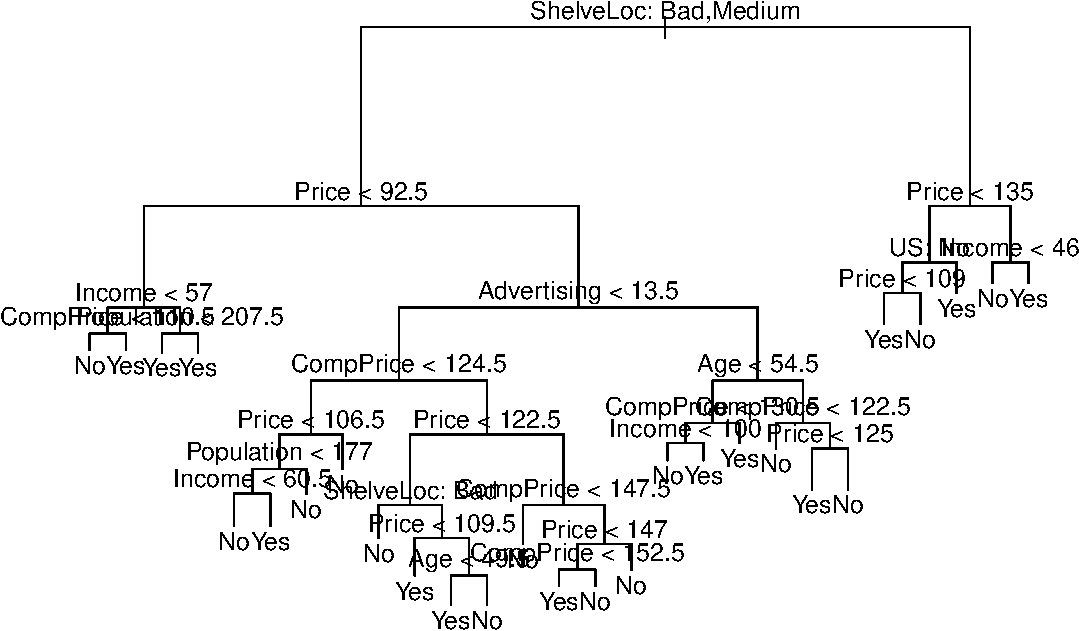
\includegraphics{ch08_lab_files/figure-latex/carseats-tree-plot-1} \end{center}

The plot should be read from the root downward. At each internal node,
the condition sends an observation left or right. A terminal node gives
the final class prediction and its estimated class probabilities.

\subsection{Cross-validation and
pruning}\label{cross-validation-and-pruning}

A tree with too many terminal nodes has high variance, while a tree that
is too small may have high bias. Cost-complexity pruning makes this
tradeoff explicit. For a subtree \(T\), a common objective is

\[
R_\alpha(T) = R(T) + \alpha |T|,
\]

where \(R(T)\) measures the tree's training misclassification error,
\(|T|\) is the number of terminal nodes, and \(\alpha \geq 0\) penalizes
complexity. A larger \(\alpha\) favours a smaller tree.

Cross-validation estimates which tree size is likely to perform best on
new data. Here we use misclassification error as the cross-validation
criterion.

\begin{Shaded}
\begin{Highlighting}[]
\FunctionTok{set.seed}\NormalTok{(}\DecValTok{1}\NormalTok{)}
\NormalTok{cv.carseats }\OtherTok{\textless{}{-}} \FunctionTok{cv.tree}\NormalTok{(tree.carseats, }\AttributeTok{FUN =}\NormalTok{ prune.misclass)}
\NormalTok{cv.carseats}
\end{Highlighting}
\end{Shaded}

\begin{verbatim}
## $size
##  [1] 27 26 24 22 19 17 14 12  7  6  5  3  2  1
## 
## $dev
##  [1] 106 108 110 106 105 102 102 102 110 108 115 115 117 164
## 
## $k
##  [1]      -Inf  0.000000  0.500000  1.000000  1.333333  1.500000  1.666667
##  [8]  2.500000  3.800000  4.000000  5.000000  7.500000 18.000000 47.000000
## 
## $method
## [1] "misclass"
## 
## attr(,"class")
## [1] "prune"         "tree.sequence"
\end{verbatim}

\begin{Shaded}
\begin{Highlighting}[]
\FunctionTok{plot}\NormalTok{(cv.carseats}\SpecialCharTok{$}\NormalTok{size, cv.carseats}\SpecialCharTok{$}\NormalTok{dev, }\AttributeTok{type =} \StringTok{"b"}\NormalTok{,}
     \AttributeTok{xlab =} \StringTok{"Number of terminal nodes"}\NormalTok{,}
     \AttributeTok{ylab =} \StringTok{"Cross{-}validated misclassification error"}\NormalTok{,}
     \AttributeTok{main =} \StringTok{"Choosing the classification{-}tree size"}\NormalTok{)}
\end{Highlighting}
\end{Shaded}

\begin{center}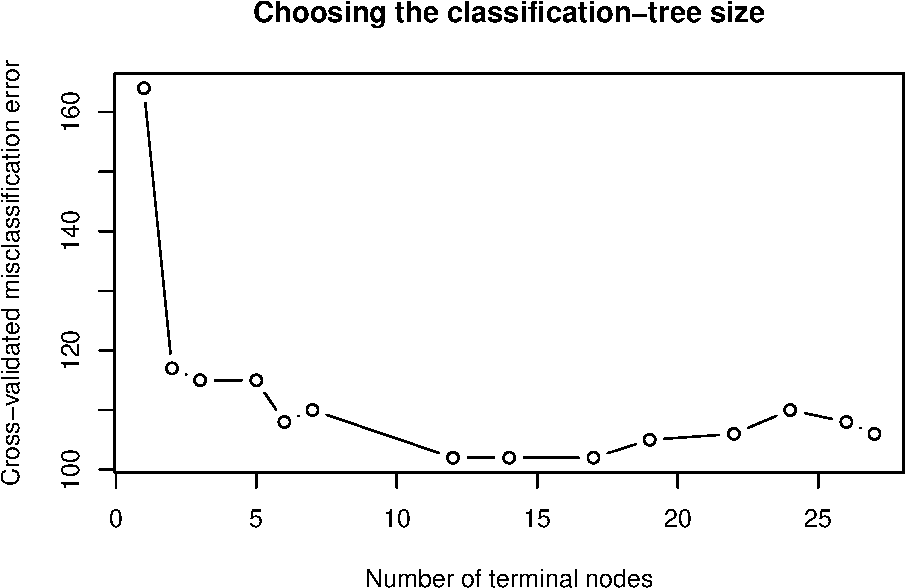
\includegraphics{ch08_lab_files/figure-latex/carseats-cv-1} \end{center}

The lowest point is the cross-validation choice. Because
cross-validation is random, a different seed can move the minimum
slightly; the important idea is that tree size is selected using
held-out predictions rather than training error alone.

\begin{Shaded}
\begin{Highlighting}[]
\NormalTok{prune.carseats }\OtherTok{\textless{}{-}} \FunctionTok{prune.misclass}\NormalTok{(tree.carseats,}
                                 \AttributeTok{best =}\NormalTok{ cv.carseats}\SpecialCharTok{$}\NormalTok{size[}\FunctionTok{which.min}\NormalTok{(cv.carseats}\SpecialCharTok{$}\NormalTok{dev)])}
\FunctionTok{summary}\NormalTok{(prune.carseats)}
\end{Highlighting}
\end{Shaded}

\begin{verbatim}
## 
## Classification tree:
## snip.tree(tree = tree.carseats, nodes = c(9L, 22L, 7L, 8L, 20L, 
## 6L))
## Variables actually used in tree construction:
## [1] "ShelveLoc"   "Price"       "Income"      "Advertising" "CompPrice"  
## [6] "Age"        
## Number of terminal nodes:  17 
## Residual mean deviance:  0.6632 = 254 / 383 
## Misclassification error rate: 0.115 = 46 / 400
\end{verbatim}

\begin{Shaded}
\begin{Highlighting}[]
\FunctionTok{plot}\NormalTok{(prune.carseats)}
\FunctionTok{text}\NormalTok{(prune.carseats, }\AttributeTok{pretty =} \DecValTok{0}\NormalTok{)}
\end{Highlighting}
\end{Shaded}

\begin{center}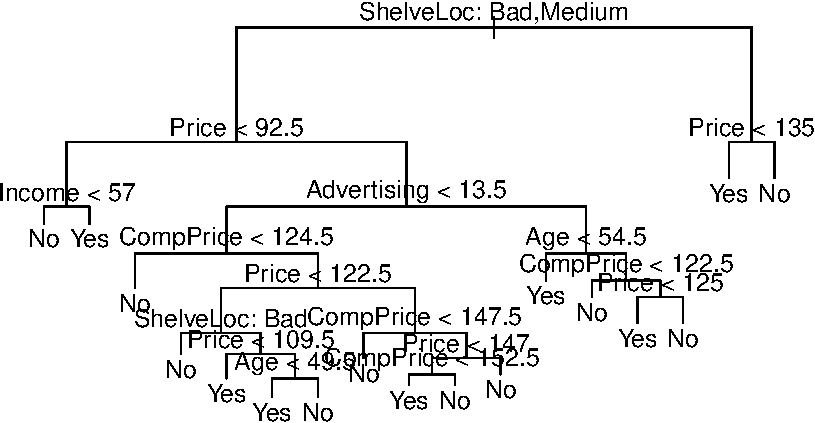
\includegraphics{ch08_lab_files/figure-latex/carseats-prune-1} \end{center}

Pruning usually produces a simpler tree. Simplicity is useful for
interpretation, but it is not automatically optimal; the
cross-validation estimate is the evidence used to choose the amount of
pruning.

\section{Regression Trees}\label{regression-trees}

\subsection{\texorpdfstring{The \texttt{Hitters}
data}{The Hitters data}}\label{the-hitters-data}

We now predict a quantitative response: baseball players' salaries. The
regression-tree analogue of a classification tree assigns a constant
prediction to every terminal node, usually the mean response of the
training observations in that node.

A regression tree chooses splits to reduce residual sum of squares
(RSS):

\[
\operatorname{RSS}(T) = \sum_{m=1}^{|T|}
  \sum_{i:x_i \in R_m}(y_i-\hat y_{R_m})^2,
\]

where \(R_m\) is a terminal region and \(\hat y_{R_m}\) is the mean
response in that region. Again, an extremely large tree can reduce
training RSS while performing poorly on new observations.

\begin{Shaded}
\begin{Highlighting}[]
\FunctionTok{data}\NormalTok{(Hitters)}
\NormalTok{Hitters }\OtherTok{\textless{}{-}} \FunctionTok{na.omit}\NormalTok{(Hitters)}

\FunctionTok{set.seed}\NormalTok{(}\DecValTok{1}\NormalTok{)}
\NormalTok{train }\OtherTok{\textless{}{-}} \FunctionTok{sample}\NormalTok{(}\DecValTok{1}\SpecialCharTok{:}\FunctionTok{nrow}\NormalTok{(Hitters), }\FunctionTok{nrow}\NormalTok{(Hitters) }\SpecialCharTok{/} \DecValTok{2}\NormalTok{)}
\NormalTok{Hitters.train }\OtherTok{\textless{}{-}}\NormalTok{ Hitters[train, ]}
\NormalTok{Hitters.test }\OtherTok{\textless{}{-}}\NormalTok{ Hitters[}\SpecialCharTok{{-}}\NormalTok{train, ]}
\end{Highlighting}
\end{Shaded}

\begin{Shaded}
\begin{Highlighting}[]
\NormalTok{tree.hitters }\OtherTok{\textless{}{-}} \FunctionTok{tree}\NormalTok{(Salary }\SpecialCharTok{\textasciitilde{}}\NormalTok{ ., }\AttributeTok{data =}\NormalTok{ Hitters.train)}
\FunctionTok{summary}\NormalTok{(tree.hitters)}
\end{Highlighting}
\end{Shaded}

\begin{verbatim}
## 
## Regression tree:
## tree(formula = Salary ~ ., data = Hitters.train)
## Variables actually used in tree construction:
## [1] "CRBI"    "CHits"   "Walks"   "CAtBat"  "CWalks"  "Runs"    "PutOuts"
## [8] "HmRun"  
## Number of terminal nodes:  10 
## Residual mean deviance:  58340 = 7060000 / 121 
## Distribution of residuals:
##    Min. 1st Qu.  Median    Mean 3rd Qu.    Max. 
## -450.90 -103.70  -16.21    0.00   74.54 1525.00
\end{verbatim}

\begin{Shaded}
\begin{Highlighting}[]
\FunctionTok{plot}\NormalTok{(tree.hitters)}
\FunctionTok{text}\NormalTok{(tree.hitters, }\AttributeTok{pretty =} \DecValTok{0}\NormalTok{)}
\end{Highlighting}
\end{Shaded}

\begin{center}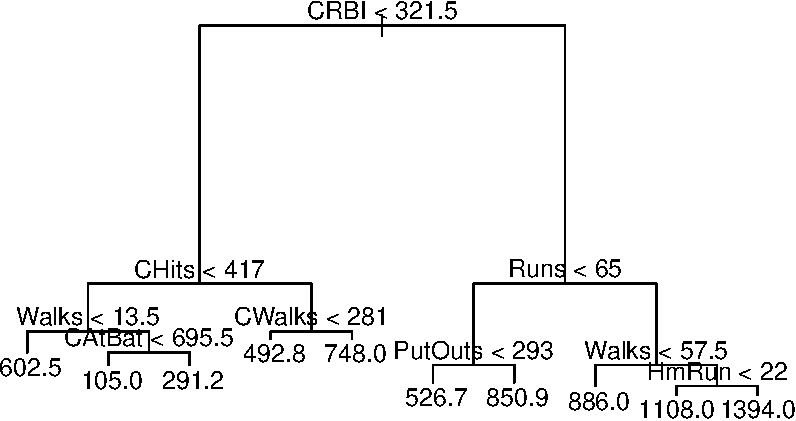
\includegraphics{ch08_lab_files/figure-latex/hitters-tree-1} \end{center}

The first split is the predictor that gives the largest immediate
reduction in RSS under the algorithm's greedy search. Later splits
represent interactions: their meaning is conditional on the decisions
made higher in the tree.

\subsection{Cross-validation and a test-set
check}\label{cross-validation-and-a-test-set-check}

\begin{Shaded}
\begin{Highlighting}[]
\FunctionTok{set.seed}\NormalTok{(}\DecValTok{1}\NormalTok{)}
\NormalTok{cv.hitters }\OtherTok{\textless{}{-}} \FunctionTok{cv.tree}\NormalTok{(tree.hitters)}
\FunctionTok{plot}\NormalTok{(cv.hitters}\SpecialCharTok{$}\NormalTok{size, cv.hitters}\SpecialCharTok{$}\NormalTok{dev, }\AttributeTok{type =} \StringTok{"b"}\NormalTok{,}
     \AttributeTok{xlab =} \StringTok{"Number of terminal nodes"}\NormalTok{,}
     \AttributeTok{ylab =} \StringTok{"Cross{-}validated RSS"}\NormalTok{,}
     \AttributeTok{main =} \StringTok{"Choosing the regression{-}tree size"}\NormalTok{)}
\end{Highlighting}
\end{Shaded}

\begin{center}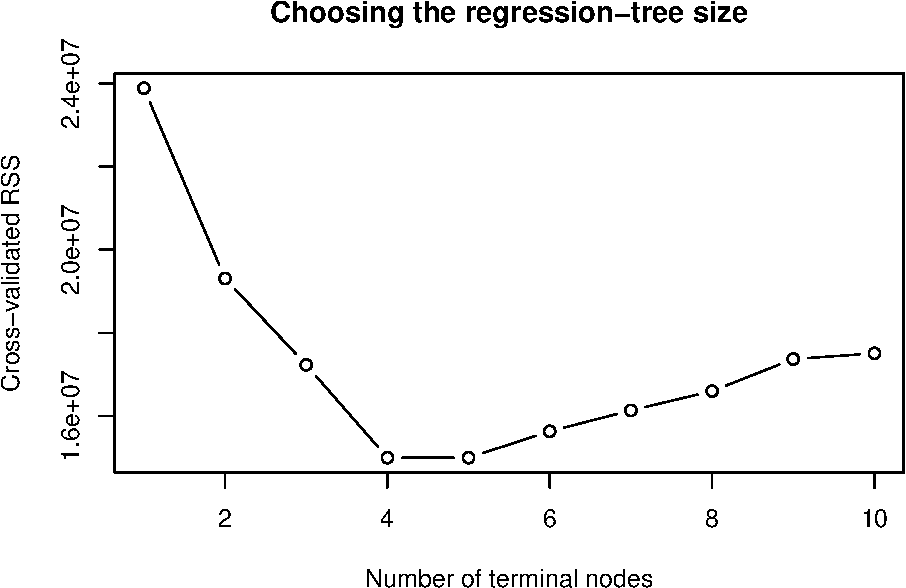
\includegraphics{ch08_lab_files/figure-latex/hitters-cv-1} \end{center}

\begin{Shaded}
\begin{Highlighting}[]
\NormalTok{prune.hitters }\OtherTok{\textless{}{-}} \FunctionTok{prune.tree}\NormalTok{(tree.hitters,}
                            \AttributeTok{best =}\NormalTok{ cv.hitters}\SpecialCharTok{$}\NormalTok{size[}\FunctionTok{which.min}\NormalTok{(cv.hitters}\SpecialCharTok{$}\NormalTok{dev)])}
\FunctionTok{summary}\NormalTok{(prune.hitters)}
\end{Highlighting}
\end{Shaded}

\begin{verbatim}
## 
## Regression tree:
## snip.tree(tree = tree.hitters, nodes = c(5L, 15L, 6L, 4L))
## Variables actually used in tree construction:
## [1] "CRBI"  "CHits" "Runs"  "Walks"
## Number of terminal nodes:  5 
## Residual mean deviance:  74730 = 9416000 / 126 
## Distribution of residuals:
##    Min. 1st Qu.  Median    Mean 3rd Qu.    Max. 
## -451.90 -153.10  -41.82    0.00  100.70 1891.00
\end{verbatim}

We evaluate the unpruned and pruned models on the same test set. Test
error is an estimate of future prediction error because these
observations were not used to fit the tree.

\begin{Shaded}
\begin{Highlighting}[]
\NormalTok{pred.tree }\OtherTok{\textless{}{-}} \FunctionTok{predict}\NormalTok{(tree.hitters, Hitters.test)}
\NormalTok{pred.pruned }\OtherTok{\textless{}{-}} \FunctionTok{predict}\NormalTok{(prune.hitters, Hitters.test)}

\NormalTok{mse.tree }\OtherTok{\textless{}{-}} \FunctionTok{mean}\NormalTok{((pred.tree }\SpecialCharTok{{-}}\NormalTok{ Hitters.test}\SpecialCharTok{$}\NormalTok{Salary)}\SpecialCharTok{\^{}}\DecValTok{2}\NormalTok{)}
\NormalTok{mse.pruned }\OtherTok{\textless{}{-}} \FunctionTok{mean}\NormalTok{((pred.pruned }\SpecialCharTok{{-}}\NormalTok{ Hitters.test}\SpecialCharTok{$}\NormalTok{Salary)}\SpecialCharTok{\^{}}\DecValTok{2}\NormalTok{)}

\FunctionTok{c}\NormalTok{(}\AttributeTok{unpruned\_MSE =}\NormalTok{ mse.tree, }\AttributeTok{pruned\_MSE =}\NormalTok{ mse.pruned)}
\end{Highlighting}
\end{Shaded}

\begin{verbatim}
## unpruned_MSE   pruned_MSE 
##     122872.5     122267.2
\end{verbatim}

The better model is the one with the smaller test MSE in this split. The
comparison also illustrates an important qualification: pruning can
improve generalisation, but the result depends on the sample split and
on the signal in the data. The purpose of the test set is to assess the
final choice, not to choose repeatedly until a favourable result
appears.

\section{Bagging and Random Forests}\label{bagging-and-random-forests}

\subsection{Why averaging trees helps}\label{why-averaging-trees-helps}

Bagging means bootstrap aggregating. We repeatedly sample \(n\)
observations with replacement, grow a tree on each bootstrap sample, and
average the predictions. For regression,

\[
\hat f_{\mathrm{bag}}(x) = \frac{1}{B}\sum_{b=1}^{B}T_b(x).
\]

If the trees have variance \(\sigma^2\) and pairwise correlation
\(\rho\), then under the usual simplifying assumptions,

\[
\operatorname{Var}\left(\frac{1}{B}\sum_{b=1}^{B}T_b(x)\right)
= \sigma^2\left(\rho + \frac{1-\rho}{B}\right).
\]

Increasing \(B\) reduces the unshared part of the variance. It cannot
remove error shared by all trees, which is why reducing tree correlation
is valuable.

\subsection{\texorpdfstring{Bagging on
\texttt{Boston}}{Bagging on Boston}}\label{bagging-on-boston}

The textbook uses the \texttt{Boston} data to compare tree ensembles for
predicting \texttt{medv}, the median value of owner-occupied homes in a
Boston suburb. We use a fixed train/test split so the models are
compared on exactly the same cases.

\begin{Shaded}
\begin{Highlighting}[]
\NormalTok{Boston }\OtherTok{\textless{}{-}}\NormalTok{ ISLR2}\SpecialCharTok{::}\NormalTok{Boston}
\FunctionTok{set.seed}\NormalTok{(}\DecValTok{1}\NormalTok{)}
\NormalTok{train }\OtherTok{\textless{}{-}} \FunctionTok{sample}\NormalTok{(}\DecValTok{1}\SpecialCharTok{:}\FunctionTok{nrow}\NormalTok{(Boston), }\FunctionTok{nrow}\NormalTok{(Boston) }\SpecialCharTok{/} \DecValTok{2}\NormalTok{)}
\NormalTok{Boston.train }\OtherTok{\textless{}{-}}\NormalTok{ Boston[train, ]}
\NormalTok{Boston.test }\OtherTok{\textless{}{-}}\NormalTok{ Boston[}\SpecialCharTok{{-}}\NormalTok{train, ]}
\end{Highlighting}
\end{Shaded}

For bagging, \texttt{mtry\ =\ 13} allows each split to consider all
predictors. The bootstrap samples create the variation between trees.

\begin{Shaded}
\begin{Highlighting}[]
\FunctionTok{set.seed}\NormalTok{(}\DecValTok{1}\NormalTok{)}
\NormalTok{bag.boston }\OtherTok{\textless{}{-}} \FunctionTok{randomForest}\NormalTok{(}
\NormalTok{  medv }\SpecialCharTok{\textasciitilde{}}\NormalTok{ ., }\AttributeTok{data =}\NormalTok{ Boston.train,}
  \AttributeTok{mtry =} \FunctionTok{ncol}\NormalTok{(Boston.train) }\SpecialCharTok{{-}} \DecValTok{1}\NormalTok{,}
  \AttributeTok{importance =} \ConstantTok{TRUE}
\NormalTok{)}

\NormalTok{bag.pred }\OtherTok{\textless{}{-}} \FunctionTok{predict}\NormalTok{(bag.boston, Boston.test)}
\NormalTok{bag.mse }\OtherTok{\textless{}{-}} \FunctionTok{mean}\NormalTok{((bag.pred }\SpecialCharTok{{-}}\NormalTok{ Boston.test}\SpecialCharTok{$}\NormalTok{medv)}\SpecialCharTok{\^{}}\DecValTok{2}\NormalTok{)}
\NormalTok{bag.mse}
\end{Highlighting}
\end{Shaded}

\begin{verbatim}
## [1] 23.41916
\end{verbatim}

The out-of-bag estimate is produced by predicting each training
observation using only trees whose bootstrap sample did not contain that
observation. It provides an internal performance estimate without a
separate validation set.

\begin{Shaded}
\begin{Highlighting}[]
\NormalTok{bag.boston}\SpecialCharTok{$}\NormalTok{mse[}\FunctionTok{length}\NormalTok{(bag.boston}\SpecialCharTok{$}\NormalTok{mse)]}
\end{Highlighting}
\end{Shaded}

\begin{verbatim}
## [1] 11.40162
\end{verbatim}

\subsection{Random Forests}\label{random-forests}

Random Forests add a second source of randomness. At each split, only a
random subset of the predictors is considered. If the strongest
predictor is not always available, different trees are forced to explore
different structures, reducing their correlation \(\rho\).

\begin{Shaded}
\begin{Highlighting}[]
\FunctionTok{set.seed}\NormalTok{(}\DecValTok{1}\NormalTok{)}
\NormalTok{rf.boston }\OtherTok{\textless{}{-}} \FunctionTok{randomForest}\NormalTok{(}
\NormalTok{  medv }\SpecialCharTok{\textasciitilde{}}\NormalTok{ ., }\AttributeTok{data =}\NormalTok{ Boston.train,}
  \AttributeTok{mtry =} \DecValTok{6}\NormalTok{,}
  \AttributeTok{importance =} \ConstantTok{TRUE}
\NormalTok{)}

\NormalTok{rf.pred }\OtherTok{\textless{}{-}} \FunctionTok{predict}\NormalTok{(rf.boston, Boston.test)}
\NormalTok{rf.mse }\OtherTok{\textless{}{-}} \FunctionTok{mean}\NormalTok{((rf.pred }\SpecialCharTok{{-}}\NormalTok{ Boston.test}\SpecialCharTok{$}\NormalTok{medv)}\SpecialCharTok{\^{}}\DecValTok{2}\NormalTok{)}
\NormalTok{rf.mse}
\end{Highlighting}
\end{Shaded}

\begin{verbatim}
## [1] 20.06644
\end{verbatim}

\begin{Shaded}
\begin{Highlighting}[]
\FunctionTok{importance}\NormalTok{(rf.boston)}
\end{Highlighting}
\end{Shaded}

\begin{verbatim}
##           %IncMSE IncNodePurity
## crim    19.435587    1070.42307
## zn       3.091630      82.19257
## indus    6.140529     590.09536
## chas     1.370310      36.70356
## nox     13.263466     859.97091
## rm      35.094741    8270.33906
## age     15.144821     634.31220
## dis      9.163776     684.87953
## rad      4.793720      83.18719
## tax      4.410714     292.20949
## ptratio  8.612780     902.20190
## lstat   28.725343    5813.04833
\end{verbatim}

\begin{Shaded}
\begin{Highlighting}[]
\FunctionTok{varImpPlot}\NormalTok{(rf.boston)}
\end{Highlighting}
\end{Shaded}

\begin{center}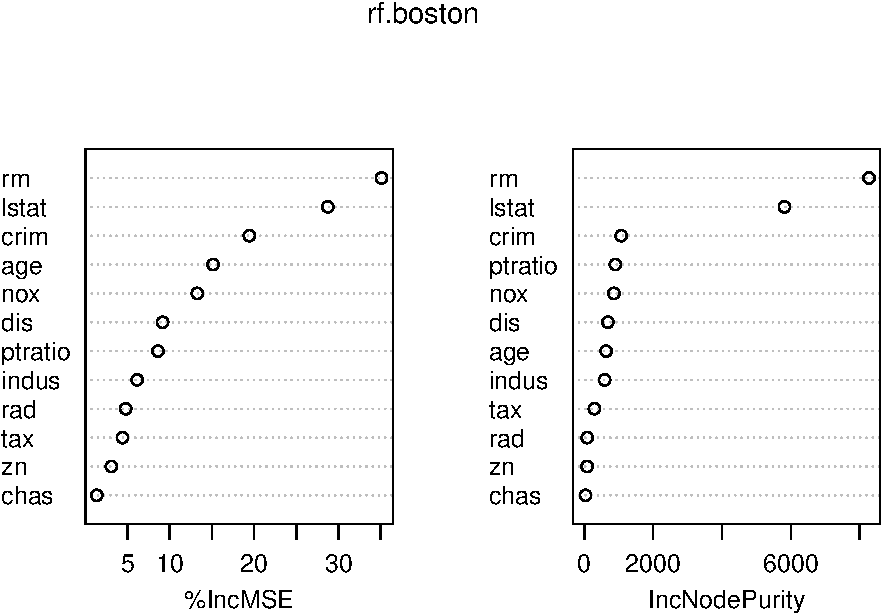
\includegraphics{ch08_lab_files/figure-latex/boston-random-forest-1} \end{center}

The test MSEs provide an empirical comparison of bagging and the Random
Forest. The Random Forest is not guaranteed to win on every split: its
design trades a little individual-tree strength for lower correlation,
and the tradeoff is data-dependent.

\begin{Shaded}
\begin{Highlighting}[]
\FunctionTok{data.frame}\NormalTok{(}
  \AttributeTok{Method =} \FunctionTok{c}\NormalTok{(}\StringTok{"Bagging"}\NormalTok{, }\StringTok{"Random Forest"}\NormalTok{),}
  \AttributeTok{Test\_MSE =} \FunctionTok{c}\NormalTok{(bag.mse, rf.mse)}
\NormalTok{)}
\end{Highlighting}
\end{Shaded}

\begin{verbatim}
##          Method Test_MSE
## 1       Bagging 23.41916
## 2 Random Forest 20.06644
\end{verbatim}

\section{Boosting}\label{boosting}

\subsection{Sequential error
correction}\label{sequential-error-correction}

Boosting does not grow independent trees and average them. Instead, it
builds an additive model one tree at a time:

\[
F_m(x) = F_{m-1}(x) + \lambda h_m(x),
\]

where \(h_m\) is a new, usually shallow, tree and \(\lambda\) is the
learning rate. For squared-error regression, the next tree is fitted to
the current residuals \(y_i-F_{m-1}(x_i)\). The new tree is therefore a
correction, not a complete model trained from scratch.

\subsection{\texorpdfstring{Gradient boosting on
\texttt{Boston}}{Gradient boosting on Boston}}\label{gradient-boosting-on-boston}

The \texttt{gbm()} implementation uses stochastic gradient boosting. Its
important controls are the number of trees, interaction depth, and
shrinkage (learning rate). A smaller learning rate usually requires more
trees but makes the updates more gradual.

\begin{Shaded}
\begin{Highlighting}[]
\FunctionTok{set.seed}\NormalTok{(}\DecValTok{1}\NormalTok{)}
\NormalTok{boost.boston }\OtherTok{\textless{}{-}} \FunctionTok{gbm}\NormalTok{(}
\NormalTok{  medv }\SpecialCharTok{\textasciitilde{}}\NormalTok{ ., }\AttributeTok{data =}\NormalTok{ Boston.train,}
  \AttributeTok{distribution =} \StringTok{"gaussian"}\NormalTok{,}
  \AttributeTok{n.trees =} \DecValTok{5000}\NormalTok{,}
  \AttributeTok{interaction.depth =} \DecValTok{4}\NormalTok{,}
  \AttributeTok{shrinkage =} \FloatTok{0.01}\NormalTok{,}
  \AttributeTok{verbose =} \ConstantTok{FALSE}
\NormalTok{)}

\FunctionTok{summary}\NormalTok{(boost.boston)}
\end{Highlighting}
\end{Shaded}

\begin{center}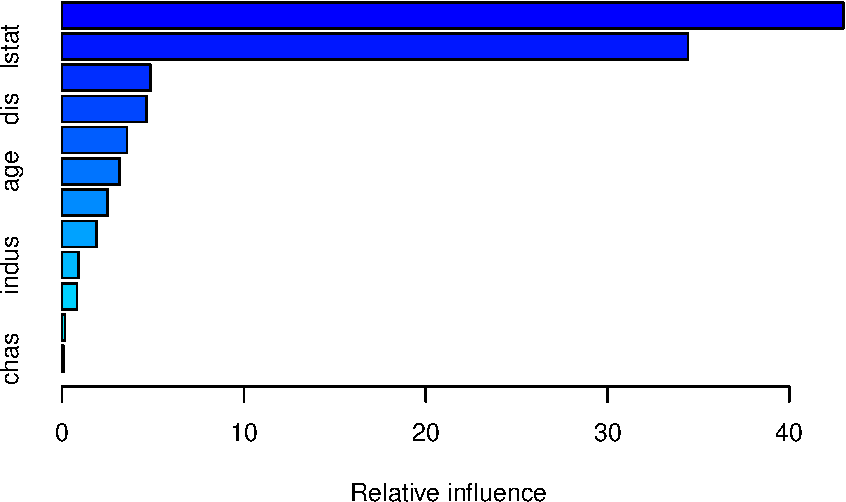
\includegraphics{ch08_lab_files/figure-latex/boston-boosting-1} \end{center}

\begin{verbatim}
##             var     rel.inf
## rm           rm 42.96709666
## lstat     lstat 34.43613309
## crim       crim  4.87078782
## dis         dis  4.63504360
## nox         nox  3.58276509
## age         age  3.17018795
## ptratio ptratio  2.51023644
## tax         tax  1.88741011
## indus     indus  0.88953756
## rad         rad  0.81391326
## zn           zn  0.15908135
## chas       chas  0.07780706
\end{verbatim}

The variable-importance plot summarizes how much each variable
contributes to reducing the loss across the boosted trees. It is a
useful descriptive tool, not proof that a variable causes the response.

\begin{Shaded}
\begin{Highlighting}[]
\FunctionTok{par}\NormalTok{(}\AttributeTok{mar =} \FunctionTok{c}\NormalTok{(}\DecValTok{5}\NormalTok{, }\DecValTok{10}\NormalTok{, }\DecValTok{4}\NormalTok{, }\DecValTok{2}\NormalTok{))}
\FunctionTok{summary}\NormalTok{(boost.boston, }\AttributeTok{las =} \DecValTok{1}\NormalTok{)}
\end{Highlighting}
\end{Shaded}

\begin{center}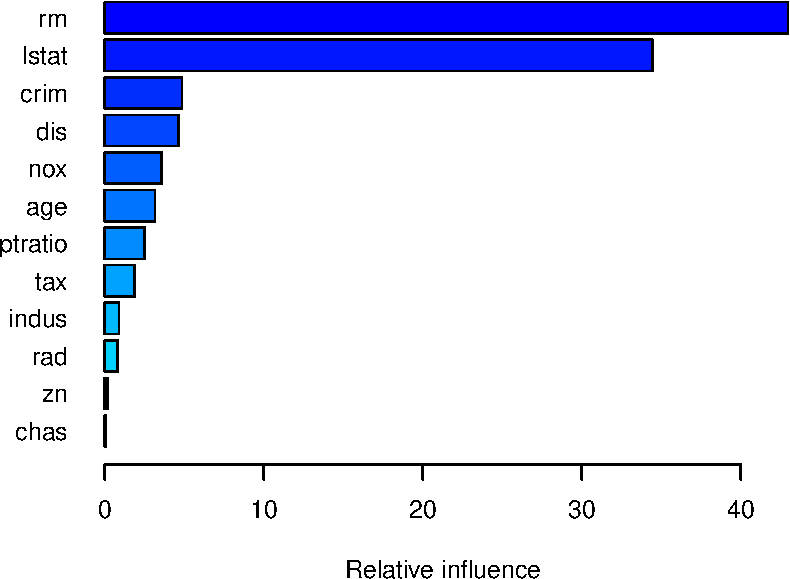
\includegraphics{ch08_lab_files/figure-latex/boston-boosting-importance-1} \end{center}

\begin{verbatim}
##             var     rel.inf
## rm           rm 42.96709666
## lstat     lstat 34.43613309
## crim       crim  4.87078782
## dis         dis  4.63504360
## nox         nox  3.58276509
## age         age  3.17018795
## ptratio ptratio  2.51023644
## tax         tax  1.88741011
## indus     indus  0.88953756
## rad         rad  0.81391326
## zn           zn  0.15908135
## chas       chas  0.07780706
\end{verbatim}

\begin{Shaded}
\begin{Highlighting}[]
\NormalTok{boost.pred }\OtherTok{\textless{}{-}} \FunctionTok{predict}\NormalTok{(boost.boston, Boston.test, }\AttributeTok{n.trees =} \DecValTok{5000}\NormalTok{)}
\NormalTok{boost.mse }\OtherTok{\textless{}{-}} \FunctionTok{mean}\NormalTok{((boost.pred }\SpecialCharTok{{-}}\NormalTok{ Boston.test}\SpecialCharTok{$}\NormalTok{medv)}\SpecialCharTok{\^{}}\DecValTok{2}\NormalTok{)}
\NormalTok{boost.mse}
\end{Highlighting}
\end{Shaded}

\begin{verbatim}
## [1] 17.24452
\end{verbatim}

\begin{Shaded}
\begin{Highlighting}[]
\NormalTok{ensemble.results }\OtherTok{\textless{}{-}} \FunctionTok{data.frame}\NormalTok{(}
  \AttributeTok{Method =} \FunctionTok{c}\NormalTok{(}\StringTok{"Bagging"}\NormalTok{, }\StringTok{"Random Forest"}\NormalTok{, }\StringTok{"Boosting"}\NormalTok{),}
  \AttributeTok{Test\_MSE =} \FunctionTok{c}\NormalTok{(bag.mse, rf.mse, boost.mse)}
\NormalTok{)}
\NormalTok{ensemble.results[}\FunctionTok{order}\NormalTok{(ensemble.results}\SpecialCharTok{$}\NormalTok{Test\_MSE), ]}
\end{Highlighting}
\end{Shaded}

\begin{verbatim}
##          Method Test_MSE
## 3      Boosting 17.24452
## 2 Random Forest 20.06644
## 1       Bagging 23.41916
\end{verbatim}

The smallest test MSE in this table is the best result for this
particular split and set of tuning choices. It should not be interpreted
as a universal ranking. In practice, the number of trees, depth,
learning rate, and feature sampling settings should be selected using
cross-validation or a validation set, and the final test set should be
used only once for the final assessment.

\section{Bayesian Additive Regression
Trees}\label{bayesian-additive-regression-trees}

Bayesian Additive Regression Trees (BART) also represent the response as
a sum of many trees:

\[
Y = \sum_{j=1}^{m} g(X; T_j, M_j) + \varepsilon,
\qquad \varepsilon \sim N(0, \sigma^2).
\]

Here \(T_j\) is the structure of tree \(j\) and \(M_j\) contains its
terminal-node values. Unlike ordinary boosting, BART puts prior
distributions on tree structures and leaf parameters, then uses
posterior sampling to represent uncertainty about the ensemble.

\begin{Shaded}
\begin{Highlighting}[]
\FunctionTok{set.seed}\NormalTok{(}\DecValTok{1}\NormalTok{)}
\NormalTok{x.train }\OtherTok{\textless{}{-}} \FunctionTok{as.matrix}\NormalTok{(Boston.train[, }\FunctionTok{setdiff}\NormalTok{(}\FunctionTok{names}\NormalTok{(Boston.train), }\StringTok{"medv"}\NormalTok{)])}
\NormalTok{y.train }\OtherTok{\textless{}{-}}\NormalTok{ Boston.train}\SpecialCharTok{$}\NormalTok{medv}
\NormalTok{x.test }\OtherTok{\textless{}{-}} \FunctionTok{as.matrix}\NormalTok{(Boston.test[, }\FunctionTok{setdiff}\NormalTok{(}\FunctionTok{names}\NormalTok{(Boston.test), }\StringTok{"medv"}\NormalTok{)])}

\NormalTok{bart.fit }\OtherTok{\textless{}{-}} \FunctionTok{wbart}\NormalTok{(}
\NormalTok{  x.train, y.train,}
  \AttributeTok{x.test =}\NormalTok{ x.test,}
  \AttributeTok{nskip =} \DecValTok{1000}\NormalTok{,}
  \AttributeTok{ndpost =} \DecValTok{2000}\NormalTok{,}
  \AttributeTok{ntree =} \DecValTok{200}
\NormalTok{)}
\end{Highlighting}
\end{Shaded}

\begin{verbatim}
## *****Into main of wbart
## *****Data:
## data:n,p,np: 253, 12, 253
## y1,yn: 0.213439, -5.486561
## x1,x[n*p]: 0.109590, 20.080000
## xp1,xp[np*p]: 0.027310, 7.880000
## *****Number of Trees: 200
## *****Number of Cut Points: 100 ... 100
## *****burn and ndpost: 1000, 2000
## *****Prior:beta,alpha,tau,nu,lambda: 2.000000,0.950000,0.795495,3.000000,3.716363
## *****sigma: 4.367914
## *****w (weights): 1.000000 ... 1.000000
## *****Dirichlet:sparse,theta,omega,a,b,rho,augment: 0,0,1,0.5,1,12,0
## *****nkeeptrain,nkeeptest,nkeeptestme,nkeeptreedraws: 2000,2000,2000,2000
## *****printevery: 100
## *****skiptr,skipte,skipteme,skiptreedraws: 1,1,1,1
## 
## MCMC
## done 0 (out of 3000)
## done 100 (out of 3000)
## done 200 (out of 3000)
## done 300 (out of 3000)
## done 400 (out of 3000)
## done 500 (out of 3000)
## done 600 (out of 3000)
## done 700 (out of 3000)
## done 800 (out of 3000)
## done 900 (out of 3000)
## done 1000 (out of 3000)
## done 1100 (out of 3000)
## done 1200 (out of 3000)
## done 1300 (out of 3000)
## done 1400 (out of 3000)
## done 1500 (out of 3000)
## done 1600 (out of 3000)
## done 1700 (out of 3000)
## done 1800 (out of 3000)
## done 1900 (out of 3000)
## done 2000 (out of 3000)
## done 2100 (out of 3000)
## done 2200 (out of 3000)
## done 2300 (out of 3000)
## done 2400 (out of 3000)
## done 2500 (out of 3000)
## done 2600 (out of 3000)
## done 2700 (out of 3000)
## done 2800 (out of 3000)
## done 2900 (out of 3000)
## time: 5s
## check counts
## trcnt,tecnt,temecnt,treedrawscnt: 2000,2000,2000,2000
\end{verbatim}

\begin{Shaded}
\begin{Highlighting}[]
\NormalTok{bart.pred }\OtherTok{\textless{}{-}} \FunctionTok{colMeans}\NormalTok{(bart.fit}\SpecialCharTok{$}\NormalTok{yhat.test)}
\NormalTok{bart.mse }\OtherTok{\textless{}{-}} \FunctionTok{mean}\NormalTok{((bart.pred }\SpecialCharTok{{-}}\NormalTok{ Boston.test}\SpecialCharTok{$}\NormalTok{medv)}\SpecialCharTok{\^{}}\DecValTok{2}\NormalTok{)}
\NormalTok{bart.mse}
\end{Highlighting}
\end{Shaded}

\begin{verbatim}
## [1] 16.0127
\end{verbatim}

The BART prediction is the posterior mean of the test predictions. Its
posterior draws also contain uncertainty information, which is a major
conceptual difference from a single fitted tree or a
point-prediction-only ensemble.

\begin{Shaded}
\begin{Highlighting}[]
\NormalTok{final.results }\OtherTok{\textless{}{-}} \FunctionTok{rbind}\NormalTok{(}
\NormalTok{  ensemble.results,}
  \FunctionTok{data.frame}\NormalTok{(}\AttributeTok{Method =} \StringTok{"BART"}\NormalTok{, }\AttributeTok{Test\_MSE =}\NormalTok{ bart.mse)}
\NormalTok{)}
\NormalTok{final.results[}\FunctionTok{order}\NormalTok{(final.results}\SpecialCharTok{$}\NormalTok{Test\_MSE), ]}
\end{Highlighting}
\end{Shaded}

\begin{verbatim}
##          Method Test_MSE
## 4          BART 16.01270
## 3      Boosting 17.24452
## 2 Random Forest 20.06644
## 1       Bagging 23.41916
\end{verbatim}

\section{Conclusion}\label{conclusion}

A single tree gives an interpretable sequence of decisions, but its
structure can be unstable. Pruning controls that instability by
selecting a smaller subtree. Bagging reduces variance by averaging trees
grown on bootstrap samples. Random Forests improve the averaging
strategy by also reducing the correlation between trees through random
feature selection. Boosting follows a different path: it grows trees
sequentially, with each tree correcting the current ensemble. BART
extends the additive-tree idea with Bayesian priors and posterior
uncertainty.

The main lesson is not that one method always wins. The appropriate
method depends on the response type, the signal-to-noise ratio, the
amount of tuning available, and whether interpretability or predictive
accuracy is the primary goal. A fair comparison requires the same data
split or resampling scheme, careful control of tuning, and a final
evaluation on observations not used to fit the chosen model.

\end{document}
